\documentclass{beamer}

\newcommand{\lesson}{{\tt ArrayList}}


\newcommand{\course}{Introduction to Object-Oriented Programming}
\subject{\course}
\title[\lesson]{\course}
\subtitle{\lesson}

\author[CS 1331]
{Christopher Simpkins \\\texttt{chris.simpkins@gatech.edu}}
\institute[Georgia Tech]

\date[]{}

\newcommand{\link}[2]{\href{#1}{\textcolor{blue}{\underline{#2}}}}
\newcommand{\code}{http://cs1331.gatech.edu/code}

\usepackage{colortbl}

% If you have a file called "university-logo-filename.xxx", where xxx
% is a graphic format that can be processed by latex or pdflatex,
% resp., then you can add a logo as follows:

% \pgfdeclareimage[width=0.6in]{coc-logo}{cc_2012_logo}
% \logo{\pgfuseimage{coc-logo}}

\mode<presentation>
{
  \usetheme{Berlin}
  \useoutertheme{infolines}

  % or ...

 \setbeamercovered{transparent}
  % or whatever (possibly just delete it)
}

\usepackage{tikz}
% Optional PGF libraries
\usepackage{pgflibraryarrows}
\usepackage{pgflibrarysnakes}
\usepackage{pgfplots}
\usepackage{fancybox}
\usepackage{listings}
\usepackage{hyperref}
\hypersetup{colorlinks=true,urlcolor=blue}
\usepackage[english]{babel}
% or whatever

\usepackage[latin1]{inputenc}
% or whatever

\usepackage{times}
\usepackage[T1]{fontenc}
% Or whatever. Note that the encoding and the font should match. If T1
% does not look nice, try deleting the line with the fontenc.


\usepackage{listings}

% "define" Scala
\lstdefinelanguage{scala}{
  morekeywords={abstract,case,catch,class,def,%
    do,else,extends,false,final,finally,%
    for,if,implicit,import,match,mixin,%
    new,null,object,override,package,%
    private,protected,requires,return,sealed,%
    super,this,throw,trait,true,try,%
    type,val,var,while,with,yield},
  otherkeywords={=>,<-,<\%,<:,>:,\#,@},
  sensitive=true,
  morecomment=[l]{//},
  morecomment=[n]{/*}{*/},
  morestring=[b]",
  morestring=[b]',
  morestring=[b]""",
}

\usepackage{color}
\definecolor{dkgreen}{rgb}{0,0.6,0}
\definecolor{gray}{rgb}{0.5,0.5,0.5}
\definecolor{mauve}{rgb}{0.58,0,0.82}

% Default settings for code listings
\lstset{frame=tb,
  language=scala,
  aboveskip=2mm,
  belowskip=2mm,
  showstringspaces=false,
  columns=flexible,
  basicstyle={\scriptsize\ttfamily},
  numbers=none,
  numberstyle=\tiny\color{gray},
  keywordstyle=\color{blue},
  commentstyle=\color{dkgreen},
  stringstyle=\color{mauve},
  frame=single,
  breaklines=true,
  breakatwhitespace=true,
  keepspaces=true
  %tabsize=3
}


% \beamerdefaultoverlayspecification{<+->}

\begin{document}

\begin{frame}
  \titlepage
\end{frame}

%------------------------------------------------------------------------
\begin{frame}[fragile]{Java Collections and {\tt java.util.ArrayList}}

\begin{itemize}
\item The Java collections hierarchy
\item Arrays and {\tt ArrayList}
\item ArrayList basics
\item Primitives in Collections
\item Generics
\item The {\tt equals} Method and Collections
\end{itemize}


\end{frame}
%------------------------------------------------------------------------

%------------------------------------------------------------------------
\begin{frame}[fragile]{Java Collections}

\begin{center}
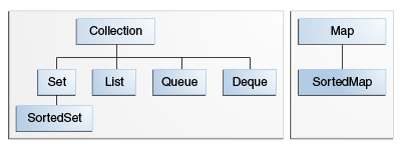
\includegraphics[width=4in]{colls-coreInterfaces.png}
\end{center}

{\tt ArralyList} and {\tt LinkedList} are the two basic {\tt List} implementations provided in the Java standard library.\footnote{{\tt Vector} also implements {\tt List} and can be thought of as a synchronized version of {\tt ArrayList}.  You don't need {\tt Vector} if you're not writing multithreaded code.  Using {\tt Vector} in single-threaded code will decrease performance.}  The concepts we'll learn for {\tt ArrayList} apply to all of Java's collection classes.

\end{frame}
%------------------------------------------------------------------------


%------------------------------------------------------------------------
\begin{frame}[fragile]{Arrays and {\tt ArrayList}}


\begin{itemize}
\item Arrays are fixed-size collections of any data types, including primitives
\item {\tt ArrayList}s are dynamically-allocated (i.e., automatically resized) collections of reference types (not primitives - but we'll talk about autoboxing).
\item {\tt ArrayList}s use arrays internally, but this isn't important to know for basic use.
\end{itemize}


\end{frame}
%------------------------------------------------------------------------

%------------------------------------------------------------------------
\begin{frame}[fragile]{{\tt ArrayList} Basics}


Create an {\tt ArrayList} with operator {\tt new}:
\begin{lstlisting}[language=Java]
  ArrayList tasks = new ArrayList();
\end{lstlisting}
Add items with {\tt add()}:
\begin{lstlisting}[language=Java]
  tasks.add("Eat");
  tasks.add("Sleep");
  tasks.add("Code");
\end{lstlisting}
Traverse with for-each loop:
\begin{lstlisting}[language=Java]
  for (Object task: tasks) {
      System.out.println(task);
  }
\end{lstlisting}

Note that the for-each loop implicitly uses an iterator.

\end{frame}
%------------------------------------------------------------------------

%------------------------------------------------------------------------
\begin{frame}[fragile]{Iterators}


Iterators are objects that provide access to the objects in a collection.  In Java iterators are represented by the {\tt Iterator} interface, which contains three methods:
\begin{itemize}
\item {\tt hasNext()} returns true if the iteration has more elements.
\item {\tt next()} returns the next element in the iteration.
\item {\tt remove()} removes from the underlying collection the last element returned by the iterator (optional operation).
\end{itemize}

The most basic and common use of an iterator is to traverse a collection (visit all the elements in a collection):
\begin{lstlisting}[language=Java]
ArrayList tasks = new ArrayList();
// ...
Iterator tasksIter = tasks.iterator();
while (tasksIter.hasNext()) {
    Object task = tasksIter.next();
    System.out.println(task);
}
\end{lstlisting}
See \link{\code/ArrayListBasics.java}{ArrayListBasics.java} for more.

\end{frame}
%------------------------------------------------------------------------

%------------------------------------------------------------------------
\begin{frame}[fragile]{Primitives in Collections}

{\tt ArrayList}s can only hold reference types.  So you must use wrapper classes for primitives:
\begin{lstlisting}[language=Java]
  ArrayList ints = new ArrayList();
  ints.add(new Integer(42));
\end{lstlisting}
Java auto-boxes primitives when adding to a collection:
\begin{lstlisting}[language=Java]
  ints.add(99);
\end{lstlisting}
But auto-unboxing can't be done when retrieving from an untyped collection:
\begin{lstlisting}[language=Java]
  int num = ints.get(0); // won't compile
\end{lstlisting}
The old way to handle this with untyped collections is to cast it:
\begin{lstlisting}[language=Java]
int num = (Integer) ints.get(0); // auto-unboxing on assignment to int
\end{lstlisting}
We'll see a better way to handle this with generics.

See \link{\code/ArrayListPrimitivesDemo.java}{ArrayListPrimitivesDemo.java} for more.
\end{frame}
%------------------------------------------------------------------------

%------------------------------------------------------------------------
\begin{frame}[fragile]{Generics}


Did you notice the warning when we compile {\tt ArrayListBasics.java}?
\begin{lstlisting}[language=bash]
$ javac ArrayListBasics.java
Note: ArrayListBasics.java uses unchecked or unsafe operations.
Note: Recompile with -Xlint:unchecked for details.
\end{lstlisting}
% $
Java issues this warning because {\tt ArrayList} (and the other collecttion classes in the Java library) is a {\it parameterized type} and we used {\tt ArrayList} without a type parameter.  The full class name is {\tt ArrayList<E>}.
\begin{itemize}
\item {\tt E} is a {\it type parameter}, which can be any class name (not a primitive type).
\item {\tt ArrayList<E>} is a {\it parameterized type}
\item {\tt E} tells the compiler which types are stored in the collection.
\end{itemize}
So the compiler is warning us that we're not using the type parameter and thus missing out on static type-checking.

\end{frame}
%------------------------------------------------------------------------

%------------------------------------------------------------------------
\begin{frame}[fragile]{Using Generics}


Supply a type argument in the angle brackets.  Read {\tt ArrayList<String>} as ``ArrayList of String''
\begin{lstlisting}[language=Java]
  ArrayList<String> strings = new ArrayList<String>();
  strings.add("Helluva"); strings.add("Engineer!");
\end{lstlisting}
If we try to add an object that isn't a {\tt String}, we get a compile error:
\begin{lstlisting}[language=Java]
  Integer BULL_DOG = Integer.MIN_VALUE;
  strings.add(BULL_DOG); // Won't compile
\end{lstlisting}

With a typed collection, we get autoboxing on insertion {\it and} retrieval:

\begin{lstlisting}[language=Java]
  ArrayList<Integer> ints = new ArrayList<>();
  ints.add(42);
  int num = ints.get(0);
\end{lstlisting}
Notice that we didn't need to supply the type parameter in the creation expression above.  Java inferred the type parameter from the declaration. (Note: this only works in Java 7 and above.)

See \link{\code/ArrayListGenericsDemo.java}{ArrayListGenericsDemo.java} for more.

\end{frame}
%------------------------------------------------------------------------

%------------------------------------------------------------------------
\begin{frame}[fragile]{The {\tt equals} Method and Collections}



\begin{itemize}
\item A class whose instances will be stored in a collection must have a properly implemented {\tt equals} method.
\item The {\tt contains} method in collections uses the {\tt equals} method in the stored objects.
\item The default implementation of {\tt equals} (object identity - true only for same object in memory) only rarely gives correct results.
\item Note that {\tt hashcode()} also has a defualt implementation that uses the object's memory address.  As a rule, whenever you override {\tt equals}, you should also override {\tt hashcode}\footnote{{\tt hashcode()} is used in objects that are keys in {\tt Map}s.  You'll learn about {\tt Map}s later in the course.}.
\end{itemize}


\end{frame}
%------------------------------------------------------------------------

%------------------------------------------------------------------------
\begin{frame}[fragile]{{\tt equals} Method Examples}


In this simple class hierarchy, {\tt FoundPerson} has a properly implemented {\tt equals} method and {\tt LostPerson} does not.
\begin{lstlisting}[language=Java]
public class ArrayListEqualsDemo {
    static abstract class Person {
        public String name;
        public Person(String name) { this.name = name; }
    }
    static class LostPerson extends Person {
        public LostPerson(String name) { super(name); }
    }
    static class FoundPerson extends Person {
        public FoundPerson(String name) { super(name); }

        public boolean equals(Object other) {
            if (this == other) return true;
            if (!(other instanceof Person)) return false;
            return ((Person) other).name.equals(this.name);
        }
    }
\end{lstlisting}

Examine the code in \link{\code/ArrayListEqualsDemo.java}{ArrayListEqualsDemo.java} to see the consequences.

\end{frame}
%------------------------------------------------------------------------

%------------------------------------------------------------------------
\begin{frame}[fragile]{Closing Thoughts on Collections and {\tt ArrayList}}


\begin{itemize}
\item Collection classes are very useful - study the Java API docs to become familiar with them.
\item The concepts we just learned about {\tt ArrayList} apply to all collections.
\item In a few weeks we'll implement several basic data structures.
\begin{itemize}
\item Computer scientists need a deep understanding of data structures.
\item Application programmers should almost always use predefined data structures from the standard library.
\end{itemize}
\item For now, knowing how to use Java collections is an important skill for any Java programmer, and collections are used extensively in Swing.
\end{itemize}


\end{frame}
%------------------------------------------------------------------------


% %------------------------------------------------------------------------
% \begin{frame}[fragile]{}


% \begin{lstlisting}[language=Java]

% \end{lstlisting}

% \begin{itemize}
% \item
% \end{itemize}


% \end{frame}
% %------------------------------------------------------------------------


\end{document}
